% Regexes:
% \[(\d+(?:,\s*\d+)*)\]
% \[[0-9]+ *- *[0-9]+\]

% TODOs:
% - check that it's PI3NN and not P3INN (also in plots)


\documentclass{article}
\usepackage{graphicx}
\usepackage{listings}
\usepackage{amsmath}
\usepackage{amssymb}
\usepackage{array}
\usepackage{float}
\usepackage{geometry}
\usepackage[colorlinks=true, linkcolor=blue]{hyperref}
\usepackage{biblatex}
\usepackage{pifont}
\usepackage{xcolor}
\usepackage{booktabs} % For professional-looking tables
\addbibresource{main.bib}

\geometry{
  left=20mm,     % Left margin
  right=20mm,    % Right margin
  top=10mm,      % Top margin
  bottom=10mm,   % Bottom margin
}


\title{Sensitivity Analysis and Uncertainty Estimation of FINN}
\author{TODO}
\date{\today}

\begin{document}

\maketitle

\begin{abstract}
% TODO
% - problem statement:
% - approach:
% - key results:
% - conclusions:
\end{abstract}

\tableofcontents

\section{Introduction}

\subsection{Motivation}
Accurate prediction of contaminant transport in groundwater is crucial for effective remediation and risk assessment. Sorption, a key factor influencing contaminant migration, is often represented by retardation factors in transport models. Traditional models rely on predefined sorption isotherms (linear, Freundlich, or Langmuir) to describe the relationship between dissolved and sorbed contaminant concentrations. However, these isotherms introduce uncertainty as they may not capture complex real-world sorption behavior.

Machine learning (ML) offers a promising alternative by enabling data-driven learning of retardation factors without relying on predefined parametric models . The finite volume neural network (FINN) presented by \textcite{finn} combines the well-established finite volume method (FVM) with the flexibility of artificial neural networks (ANNs) to learn specific components of the governing partial differential equations (PDEs), including the retardation factor as a function of concentration . This hybrid modeling approach allows for capturing complex sorption behavior while maintaining numerical stability and providing scientifically interpretable results .
However, like all models, ML-based predictions are inherently uncertain due to factors such as limited training data, measurement noise, and model structure . Quantifying this uncertainty is crucial for providing reliable predictions and enabling informed decision-making in real-world applications. \textcite{finn} explores uncertainty quantification (UQ) techniques for FINN, including Bayes-by-backprop and Markov chain Monte Carlo (MCMC) methods . These methods, while effective, can be computationally expensive, especially for complex models with a large number of parameters .

This study is motivated by the need for more efficient UQ methods for ML-based retardation factor estimation. Building upon the FINN framework, this work proposes a novel UQ approach that assumes random hyperparameters of the ANN instead of random weights, as in Bayes-by-backprop. This alternative approach aims to provide significantly faster UQ estimates while achieving comparable accuracy to existing Bayesian methods. By focusing on the efficiency of UQ without sacrificing accuracy, our research aims to make ML-based modeling of contaminant transport more accessible and applicable for real-world scenarios.
% TODO: "significantly faster UQ estimates" sure? see other todos

\subsection{Background}
The transport of contaminants in groundwater is a complex process that involves various physical and chemical interactions. One crucial aspect is diffusion-sorption, where contaminants dissolved in groundwater can interact with the solid phase of the porous medium, such as clay, leading to sorption and desorption processes. This interaction significantly affects the migration and fate of contaminants.
The retardation factor ($R$) is a key parameter in diffusion-sorption models, quantifying the delay in contaminant transport caused by sorption. It represents the ratio of the contaminant's velocity in the absence of sorption to its actual velocity in the presence of sorption.

Mathematically, the diffusion-sorption process is often described by a partial differential equation (PDE) that incorporates the retardation factor. For example, Equation \eqref{eq:diff-sorpt-pde} presents a one-dimensional diffusion-sorption equation for dissolved contaminant concentration ($c$), where the retardation factor ($R$) is a function of $c$:

\begin{equation}
    \frac{\partial c}{\partial t} = \frac{D}{R(c)} \frac{\partial^2 c}{\partial x^2}
    \label{eq:diff-sorpt-pde}
\end{equation}

Here, $D$ represents the effective diffusion coefficient, $t$ is time, and $x$ is the distance along the flow path. The equation highlights that the diffusivity ($D/R(c)$) is dependent on the concentration due to the influence of the retardation factor.

Determining the retardation factor from concentration data is an inverse problem. Instead of directly solving the PDE with known parameters, the goal is to infer the unknown retardation factor function ($R(c)$) from observed concentration data. This inverse problem is challenging due to the limited availability and potential noise in the data, as well as the complexity of the underlying sorption processes. Even without noise, uniqueness is not guaranteed for implicit equations. Therefore, we empirically investigate the uniqueness of the retardation factor function given the diffusion-sorption PDE and boundary conditions in section \ref{sec:uniqueness}.

Uncertainty quantification (UQ) for neural networks is essential for providing reliable predictions and assessing the confidence in learned models. Given that neural networks learn from data, uncertainties in the data, model parameters, and model structure can propagate to the predictions.
Traditional UQ methods for neural networks, such as Bayes-by-backprop, involve treating the network weights as random variables and estimating their posterior distribution. However, these methods can be computationally expensive, especially for complex models. Our approach of considering random hyperparameters offers a potentially more efficient alternative for estimating uncertainty in the learned retardation factor.




\subsection{Problem Statement}
The diffusion-sorption process, governed by a PDE, describes contaminant transport in groundwater. Experimentally, data can be obtained from a soil cylinder, including breakthrough curves (BTCs) at a fixed location ($x=L$) over time ($t \in [0, T_{\text{end}}]$), and a concentration profile at a specific time ($t=T_{\text{end}}$) across the cylinder's length ($x \in [0,L]$). While a complete concentration field ($c(x,t)$, see Figure \ref{fig:c_diss_field_full}) would be ideal, it's practically unobtainable as measurements at all $x$ values require destructive sampling. Solving the PDE requires knowing the retardation function, $R(c)$, which quantifies sorption and is dependent on soil properties. Since $R(c)$ is typically unknown, FINN is employed to learn it from the available data. However, uncertainties arise from measurement errors in the data and non-uniqueness of the solver solution, leading to uncertainty in the learned retardation function. Therefore, the goal is to estimate a prediction interval (PI) around the learned $R(c)$ to quantify this uncertainty.

\begin{figure}
    \centering
    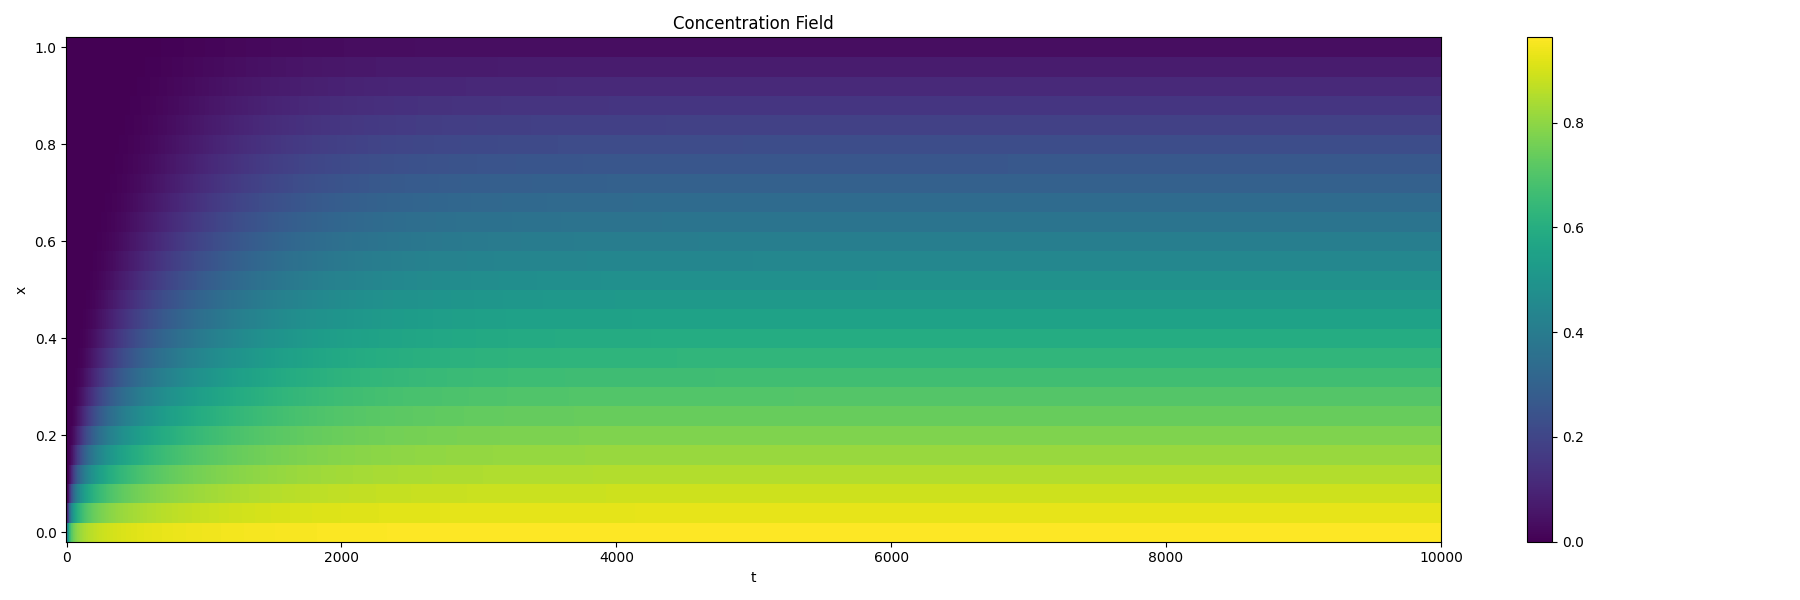
\includegraphics[width=0.9\textwidth]{figs/c_diss_field_full.png}
    \label{fig:c_diss_field_full}
\end{figure}


\subsubsection{Learning}
The goal of FINN is to learn the unknown retardation factor, $R(c)$, which is a function of the contaminant concentration, $c$. The retardation factor is a part of the diffusion-sorption equation \eqref{eq:diff-sorpt-pde} with boundary conditions:

\begin{itemize}
    \item Top Boundary: At the top end of the sample where pure-phase TCE is injected, a Dirichlet boundary condition is used:

    \begin{equation}
        c|_{x=0} = c_{sol} \quad \forall t : 0 \leq t \leq T,
    \end{equation}

    where $c_{sol}$ is the solubility limit of TCE in water and $T$ is the experiment time.

    \item Bottom Boundary: At the bottom end of the sample, which is flushed with clean water, a Cauchy boundary condition is applied:

    \begin{equation}
        c|_{x=L} = \frac{D}{Q} \frac{\partial c}{\partial x} \quad \forall t : 0 \leq t \leq T,
    \end{equation}

    where $Q$ is the flow rate of the clean water and $L$ is the sample length.
\end{itemize}

The goal is to learn $\hat{R}(x,t;\theta)$ (represented by a neural network) given the data $\mathcal{D} = \{ (x_i, t_i, c_i) \}_{i=1}^N$ which consists of concentration measurements $c_i$ at spatial positions $x_i$ and temporal points $t_i$. The network needs to be trained such that the PDE solution using $\hat{R}$ minimizes the error with respect to the data.

\subsubsection{Uncertainty Quantification}
There are two main aspects of uncertainty quantification (UQ) in this context:
\begin{enumerate}
    \item UQ for FINN output: $p(\hat{c}(x,t) | \mathcal{D})$. This represents the probability distribution of the predicted contaminant concentration $\hat{c}(x,t)$ obtained from the FINN model, given the data $\mathcal{D}$.
    \item UQ for the predicted retardation factor: $p(\hat{R}(c) | \mathcal{D})$. This is arguably more important because it represents the probability distribution of the predicted retardation factor $\hat{R}(c)$ given the data $\mathcal{D}$. This distribution helps in understanding the confidence in the estimated retardation factor.
\end{enumerate}

But there are also two types of uncertainty that have to be differentiated \cite{depeweg2018decomposition, gawlikowski2023survey}:

\begin{enumerate}
    \item Aleatoric uncertainty: This arises from inherent randomness in the data and the physical system. It is irreducible and is caused by factors such as measurement noise and variability in the system parameters.
    \item Epistemic uncertainty: This stems from limited knowledge of the model (e.g. uncertainty over its parameters). It is associated with model structure, neural network architecture, and limited training data. It quantifies the model's predictive uncertainty.
\end{enumerate}

While a clear decomposition into aleatoric and epistemic uncertainty is often not feasible, our interest extends to quantifying the overall predictive uncertainty, which encompasses both.


\subsection{Contributions of this Work}
This study addresses uncertainty quantification (UQ) in the finite volume neural network (FINN) framework when applied to a diffusion-sorption process. We begin with an empirical analysis of the uniqueness of the retardation factor, $R(c)$, which is crucial for interpreting the FINN output and forms the basis of our proposed UQ approach. We summarize FINN and PI3NN, the foundational methods used in this work. A novel framework is introduced to assess both solver and data uncertainty, allowing us to construct prediction intervals (PIs) for the retardation function. Additionally, our method performs a sensitivity analysis, exploring perturbation-sensitive directions and their impact on the FINN output. We apply the proposed framework to both synthetic and experimental datasets, comparing the results with established baselines such as the Markov Chain Monte Carlo (MCMC) approach. Our method involves using random hyperparameters of the neural network for UQ as well as random datasets. This efficient approach aims to capture both aleatoric and epistemic uncertainties, offering a computationally less expensive alternative to traditional Bayesian methods by focusing on hyperparameter variations instead of the high-dimensional weight space. % TODO: "offering a computationally less expensive" True?


\subsection{Related Work}
\subsubsection{Bayes NN}
\label{sec:bayes_nn}
% TODO: Maybe too detailed. Move some to appendix?
This section describes the baseline methodology used for comparison, which employs Bayesian inference to estimate the posterior distribution of the retardation function, $\hat{R}(c(x,t))$, parameterized by a neural network (NN). The retardation function is a function of concentration, $c$, which itself is a function of spatial position, $x$, and time, $t$. This approach updates prior beliefs about the retardation function based on observed data, $\mathcal{D}$.

\paragraph{Prior Distribution:}

A Gaussian prior distribution, $p(\theta)$, is placed over the NN parameters $\theta$, reflecting prior knowledge or assumptions. This prior is centered on the parameters $\theta_{PT}$ of a pre-trained NN, with covariance matrix $\Sigma_p = 0.05 \, I$:


\begin{equation*}
p(\theta) = \mathcal{N}(\theta | \theta_{PT}, \Sigma_p)
\end{equation*}

\paragraph{Likelihood Function:}

The likelihood function, $p(\mathcal{D} | \theta)$, quantifies the probability of observing the data $\mathcal{D}$ given a specific set of NN parameters $\theta$. We assume additive Gaussian noise with standard deviation $\sigma$ corrupts the observed concentrations. Let $c_{obs}(x,t)$ represent the observed concentration at position $x$ and time $t$, and $c_{model}(x,t; \theta)$ the concentration predicted by the model (using a FINN solver with $\hat{R}(c(x,t);\theta)$). The likelihood is:

\begin{equation}
p(\mathcal{D} | \theta) = \prod_{(x_i, t_i, c_i) \in \mathcal{D}} \frac{1}{\sqrt{2\pi \sigma^2}} \exp \left( -\frac{(c_i - c_{model}(x_i, t_i; \theta))^2}{2\sigma^2} \right)
\label{eq:likelihood}
\end{equation}

\paragraph{Posterior Distribution:}

Bayes' theorem provides the posterior distribution of the NN parameters given the data:

% TODO: is this good notation?
\begin{equation*}
p(\theta | \mathcal{D}) \propto p(\mathcal{D} | \theta) p(\theta)
\end{equation*}

\textcite{finn} compare several methods to obtain samples from this distribution, including the Metropolis-Hastings algorithm, the MALA algorithm, and the Barker method. The accepted samples $\{\theta_i\}$ from the used algorithm are then treated as draws from the posterior distribution $p(\theta | \mathcal{D})$.

\paragraph{Posterior of Retardation Function:}

Finally, the posterior distribution of the retardation function $\hat{R}(c)$ is obtained by evaluating the NN with the sampled parameters $\{\theta_i\}$:

\begin{equation*}
\{\hat{R}(c | \theta_i)\} \sim p(\hat{R}(c) | \mathcal{D})
\end{equation*}

This set of retardation function samples provides a probabilistic description of the retardation behavior, incorporating the uncertainty arising from the limited and noisy data.

Since \textcite{finn} obtain the best results with the Barker method and no burn-in period by starting from the pre-trained model, we follow their approach to have a fair comparison.



\subsection{Outline of this Work}
This work is structured as follows: Section 2 empirically investigates the uniqueness of the retardation factor inverse problem. Section 3 provides background information on the employed methods FINN and PI3NN. Section 4 details our methodology, introducing the Stochastic Perturbation Analysis of Networks (SPAN) and Data-SPAN approaches for uncertainty quantification. Section 5 describes the experimental data and setup. Section 6 presents the experimental results, including runtime comparisons and evaluations of likelihood and reliability. Section 7 discusses the findings and limitations of the proposed methods. Finally, Section 8 summarizes the work and outlines potential future research directions.



\section{Uniqueness of Inverse Problem}
\label{sec:uniqueness}
Inverse problems are not necessarily unique. Consider the simple equation $x^2 = 4$. This equation has two solutions, $x=2$ and $x=-2$. Thus, knowing the output (4) does not uniquely determine the input ($x$). This illustrates the concept of non-uniqueness in inverse problems. Instead of rigorously analyzing the problem mathematically, we perform an empirical uniqueness analysis. We achieve this by rearranging the PDE \eqref{eq:diff-sorpt-pde} to solve for $R(c)$
\begin{equation*}
    R(c) = D \frac{\partial^2 c}{\partial x^2} \frac{1}{\frac{\partial c}{\partial t}}
\end{equation*}

and substituting the synthetic data. The results, shown in Figure \ref{fig:ret_uniqueness}, suggest a unique solution for this data, except for minor numerical inaccuracies.

This allows us to attribute potential discrepancies in solutions to two primary factors: solver uncertainty and data uncertainty. We will first examine these separately and then combine them to obtain a final uncertainty quantification.


\begin{figure}
    \centering
    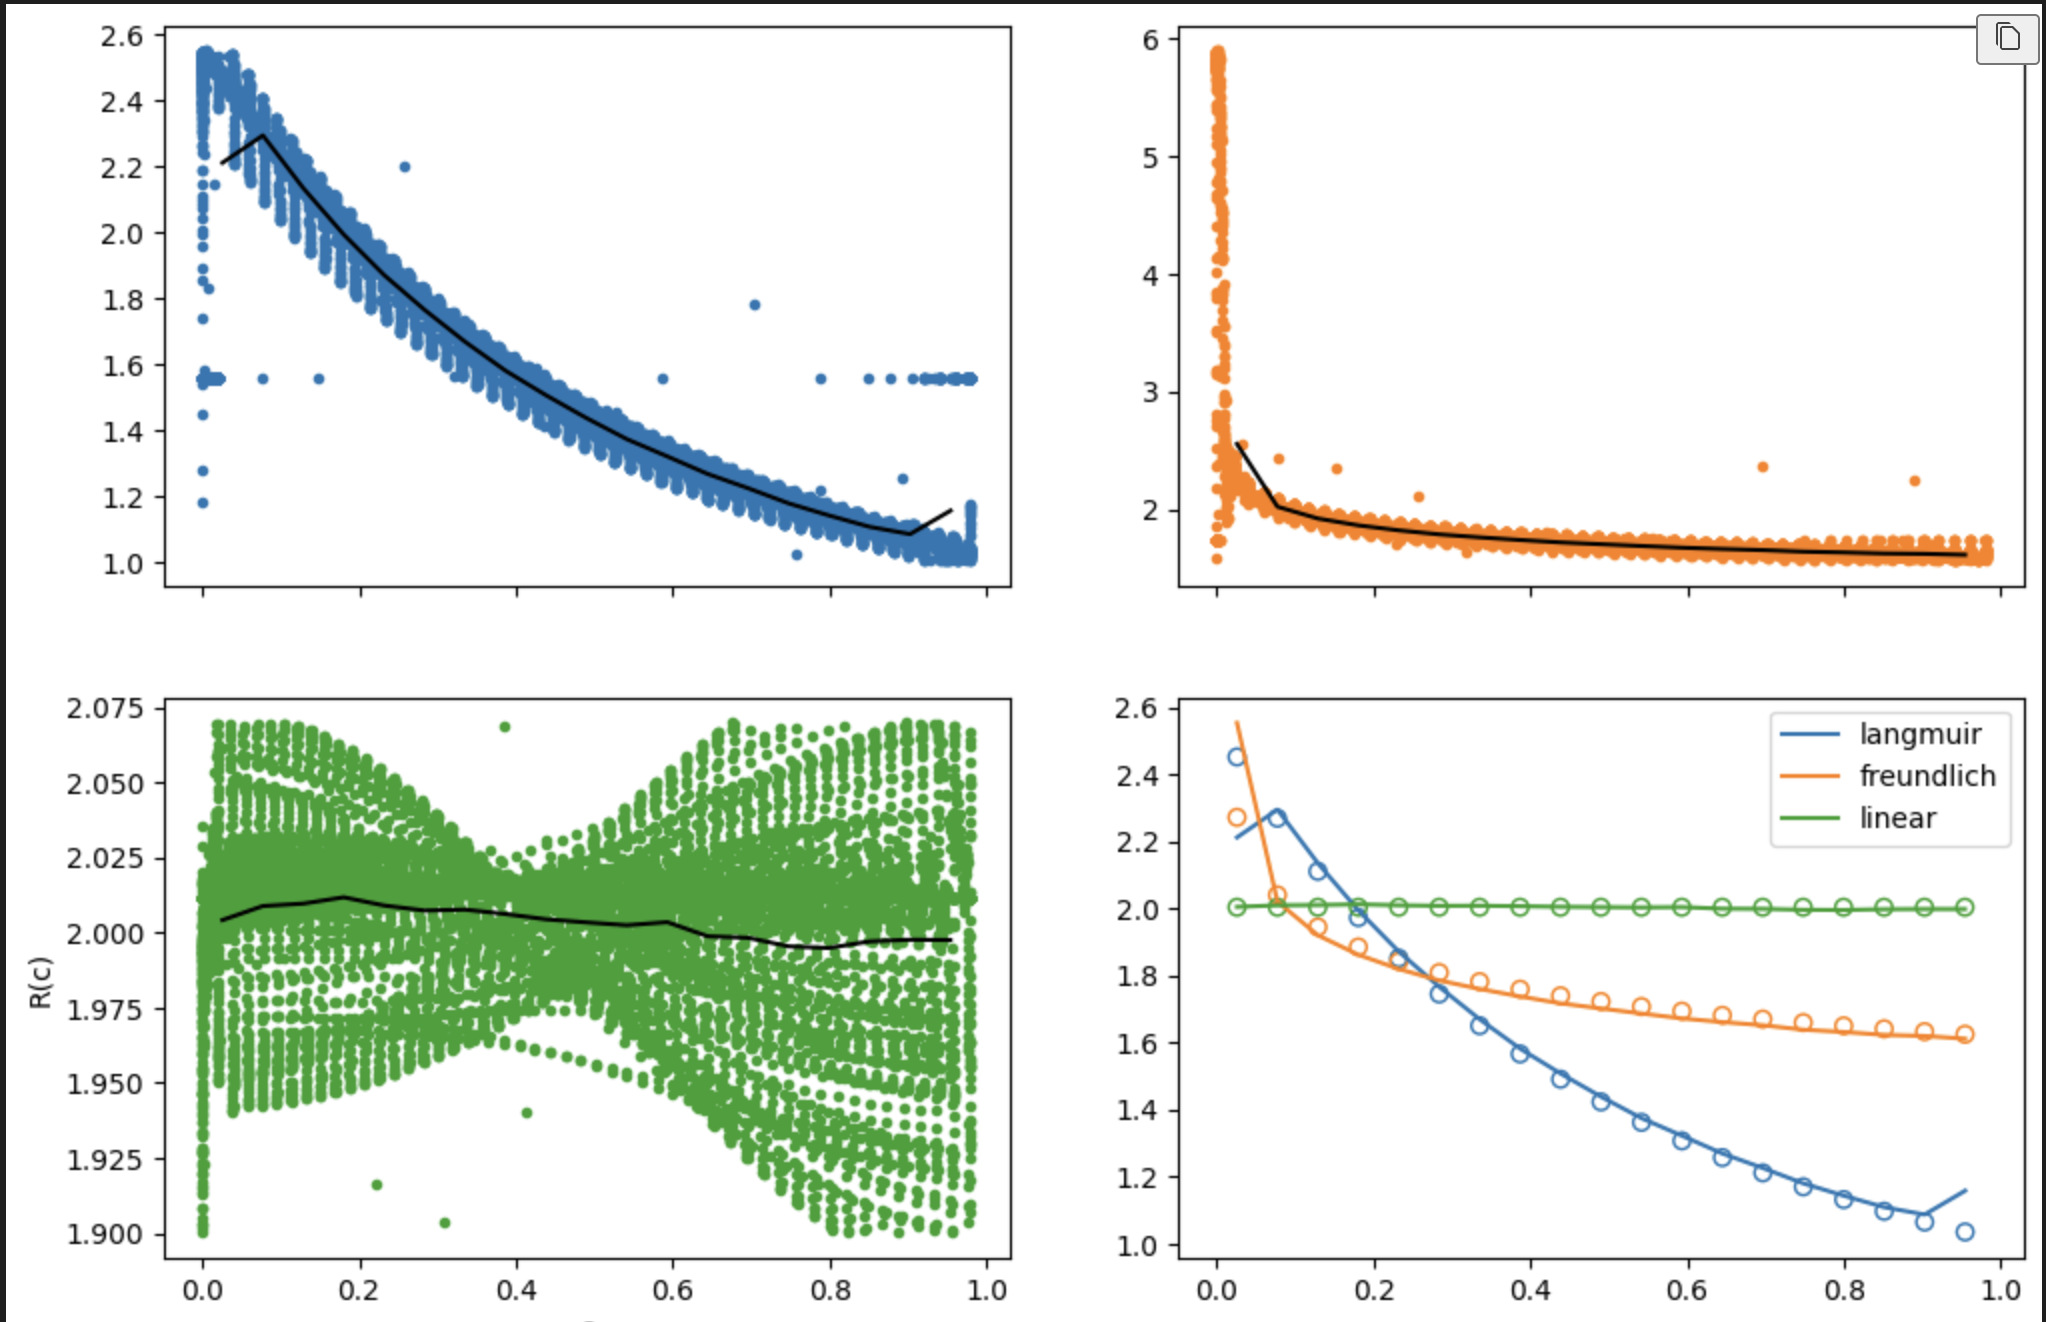
\includegraphics[width=0.9\textwidth]{figs/ret_uniqueness.png}
    \label{fig:ret_uniqueness}
    \caption{Computed retardation values (dots) and mean (black line) from analytical expression and synthetic data for linear, Freundlich and Langmuir retardations. Bottom right: Means (colored lines) and exact synthetic retardations (circles).}
\end{figure}



\section{Foundational Methods}
\subsection{FINN}

The Finite Volume Neural Network (FINN) is a specialized machine learning approach that combines the strengths of traditional numerical methods with the adaptability of neural networks to solve partial differential equations (PDEs) with unknown or uncertain components. It leverages the Finite Volume Method (FVM), dividing the problem domain into discrete control volumes. The core of FINN lies in its use of "flux kernels" $F_i$ – neural networks that learn how quantities flow between neighboring volumes. Specifically, each volume has a flux kernel composed of two subkernels, $f_{i-}$ and $f_{i+}$, one for each direction, which model these fluxes based on the concentrations in the volume and its neighbors. These subkernels consist of two parts: a "stencil" component $\Phi_N$ that approximates the FVM spatial scheme and a "diffusivity" component $\Phi_D$ that learns how the flow rate depends on the concentration itself:

\begin{align*}
    f_{i-} &= \Phi_D(c_i) \cdot \Phi_N(c_i, c_{i-1}) \\
    f_{i+} &= \Phi_D(c_i) \cdot \Phi_N(c_i, c_{i+1}).
\end{align*}

Furthermore, FINN employs "state kernels" $S_i$ that take the local concentration and calculated fluxes as input to update the concentration over time. This time evolution is governed by a Neural Ordinary Differential Equation (NODE) solver, a differentiable method that integrates seamlessly into the neural network training. By integrating FVM discretization, specialized neural network modules, and a NODE solver, FINN is capable of learning complex time-dependent spatial patterns while adhering to physical conservation laws and boundary conditions.



\subsection{PI3NN}
PI3NN (Prediction Intervals from Three Neural Networks) \cite{pi3nn} is a method for constructing prediction intervals (PIs) that uses three independently trained neural networks. It aims to provide tight, non-crossing PIs across various confidence levels without requiring retraining for each level.

The method's theoretical foundation lies in approximating the ground-truth PI bounds with a family of neural networks. Specifically, PI3NN approximates the median of the target variable, $M[y]$, and the expected deviations above and below the median, $E[(y - M[y])\mathbb{1}_{y-M[y]>0}]$ and $E[(M[y] - y)\mathbb{1}_{M[y]-y>0}]$, respectively, using three independently trained neural networks ($f_w(x)$, $u_\theta(x)$, and $l_\epsilon(x)$). These networks are trained using the standard mean squared error loss, simplifying the training process and avoiding the need for specialized loss functions and sensitive hyperparameters that often require fine-tuning in other PI methods.

Once trained, PI3NN constructs the PI bounds as linear combinations of the three networks' outputs. The coefficients of these linear combinations ($\alpha$ and $\beta$) are determined through a root-finding algorithm that ensures the desired PICP (Prediction Interval Coverage Probability) for a given confidence level $q$ ($\gamma$ in \cite{pi3nn}). This process allows for calculating PIs for multiple confidence levels without retraining the networks, offering significant computational advantages.


Figure \ref{fig:3pinn_illustration} illustrates the 6-step breakdown of the PI3NN process:
\begin{enumerate}
    \item \textbf{Learn the mean:} Train a neural network to approximate the mean of the target data.
    \item \textbf{Estimate the median:} Calculate the median by shifting the learned mean.
    \item \textbf{Calculate and split residuals:} Compute the residuals between the actual data and the estimated median, then separate these into positive and negative residuals.
    \item \textbf{Learn residuals:} Train two more neural networks, one to approximate the positive residuals and the other to approximate the negative residuals.
    \item \textbf{Construct PI:} Calculate a PI using the learned median and the learned positive and negative residuals.
    \item \textbf{Generate multiple PIs:} Use a root-finding algorithm to compute PIs for different confidence levels $q$ without retraining the networks.
\end{enumerate}


\begin{figure}
    \centering
    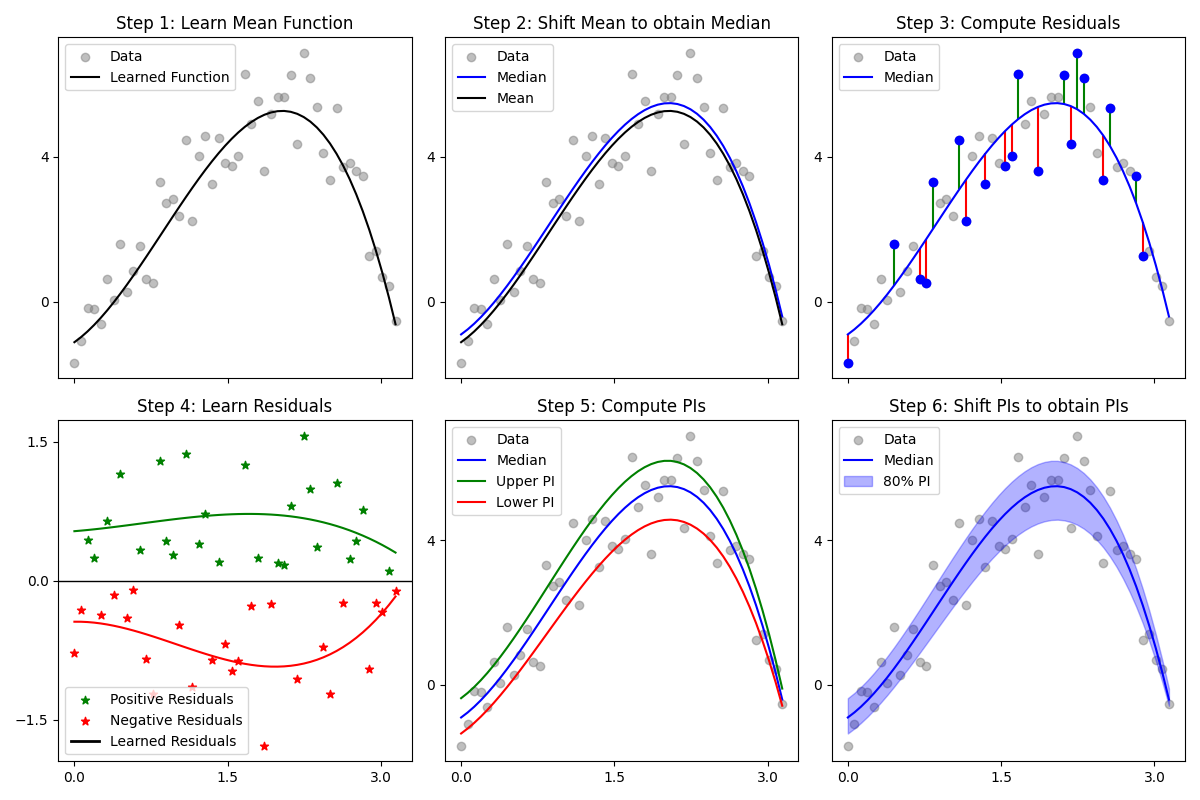
\includegraphics[width=0.9\textwidth]{figs/3pinn_illustration.png}
    \label{fig:3pinn_illustration}
    \caption{Illustration of the PI3NN method.}
\end{figure}




\section{Methodology}
\subsection{SPAN (Stochastic Perturbation Analysis of Networks)}
% TODO: SPAN = Epistemic uncertainty
Our objective is to determine the posterior predictive distribution $p(\hat{R}(c; \theta) = R(c)| \mathcal{D})$, which represents the probability of computing a specific retardation function value $R(c)$ for a given concentration $c$, based on the observed breakthrough curve data $\mathcal{D}$. We present a method that computes this distribution by marginalizing over uncertain parameters $h$ of the solver and employing an approximate likelihood function $p(\mathcal{D} | h)$ based on the same assumtions that were used for the Bayes aproach.

\subsubsection{Approximating the Posterior Predictive Distribution via Hyperparameter Marginalization}

\paragraph{Model Formulation:}

We represent our neural network as $\hat{R}(c; \theta)$, where $c$ is the input concentration and $\theta$ denotes the network's parameters (weights and biases). The parameters $\theta$ are determined by a deterministic solver $S(h, \mathcal{D})$, which takes hyperparameters $h$ and training data $\mathcal{D}$ as input. A prior distribution $p(h)$ is assigned over the hyperparameters; the exact form of $p(h)$ is not crucial, as it suffices to generate samples from it.

With $w(h) = \frac{p(\mathcal{D} | h)}{p(\mathcal{D})}$, the posterior predictive distribution can be expressed as:

\begin{align*}
p(\hat{R}(c; \theta) = R(c)| \mathcal{D}) &= \int p(\hat{R}(c; \theta) | h, \mathcal{D})\; p(h | \mathcal{D}) \, dh \\
                                          &= \int p(\hat{R}(c; \theta) | h, \mathcal{D})\; \frac{p(\mathcal{D} | h) p(h)}{p(\mathcal{D})} \, dh \\
                                          &= \int p(\hat{R}(c; \theta) | h, \mathcal{D})\; w(h)\; p(h) \, dh \\
                                          &= \int \delta(\hat{R}(c; \theta) - R(c))\; w(h)\; p(h) \, dh \\
\end{align*}

The first step is the marginalization over $h$, the second the application of Bayes' Theorem, and the last stems from the fact that the solver $\theta = S(h, \mathcal{D})$ is deterministic given $h$ and $\mathcal{D}$ and thus the distribution becomes a delta distribution.


\paragraph{Importance Sampling:}

So sampling from $p(\hat{R}(c; \theta) = R| \mathcal{D})$ becomes equivalent to sampling from $p(h)$, evaluating the solver to obtain the model parameters $\theta = S(h, \mathcal{D})$, evaluating the model $\hat{R}(c; \theta)$, and reweighting the samples with $w(h)$. This is the concept of importance sampling. To approximate the distribution, we thus have to draw $M$ samples $\{h_m\}_{m=1}^M$ from the prior distribution $p(h)$ and calculate the importance weight for each:

\begin{equation*}
w_m = \frac{p(\mathcal{D} | h_m)}{p(\mathcal{D})} \propto p(\mathcal{D} | h_m)
\end{equation*}

As $p(\mathcal{D})$ is a constant, it can be omitted, and the weights can be normalized subsequently.


\paragraph{Likelihood Computation:}
We use the same assumption about our data that the Bayesian baseline uses which results in an easy computation of the likelihood by just substituting $\theta$ with $S(h, \mathcal{D})$ in equation \eqref{eq:likelihood}:

\begin{equation*}
p(\mathcal{D} | h) = \prod_{x_i, t_i, c_i \in \mathcal{D}} \frac{1}{\sqrt{2\pi \sigma^2}} \exp \left( -\frac{(c_i - c_{model}(x_i, t_i; S(h, \mathcal{D})))^2}{2\sigma^2} \right)
\end{equation*}



\subsubsection{Data-SPAN}
% TODO: Data-SPAN = Aleatoric uncertainty
The exact same derivation can be applied when we assume a random dataset $\tilde{\mathcal{D}}$ instead of random hyperparameters $h$:

\begin{align*}
    p(\hat{R}(c; \theta) = R(c)| \mathcal{D}) &= \int p(\hat{R}(c; \theta) | \tilde{\mathcal{D}}, \mathcal{D})\; p(\tilde{\mathcal{D}} | \mathcal{D}) \, d \tilde{\mathcal{D}} \\
                                              &= \int p(\hat{R}(c; \theta) | \tilde{\mathcal{D}}, \mathcal{D})\; \frac{p(\mathcal{D} | \tilde{\mathcal{D}}) p(\tilde{\mathcal{D}})}{p(\mathcal{D})} \, d \tilde{\mathcal{D}} \\
                                              &= \int p(\hat{R}(c; \theta) | \tilde{\mathcal{D}}, \mathcal{D})\; w(\tilde{\mathcal{D}})\; p(\tilde{\mathcal{D}}) \, d \tilde{\mathcal{D}} \\
                                              &= \int \delta(\hat{R}(c; \theta) - R(c))\; w(\tilde{\mathcal{D}})\; p(\tilde{\mathcal{D}}) \, d \tilde{\mathcal{D}} \\
\end{align*}

\begin{equation*}
    p(\mathcal{D} | \tilde{\mathcal{D}}) = \prod_{x_i, t_i, c_i \in \mathcal{D}} \frac{1}{\sqrt{2\pi \sigma^2}} \exp \left( -\frac{(c_i - c_{model}(x_i, t_i; S(h, \tilde{\mathcal{D}})))^2}{2\sigma^2} \right)
\end{equation*}

\paragraph{Random Dataset Sampling:}
\label{sec:random_dataset_sampling}
To generate random datasets, we leverage PI3NN, applying it to the original breakthrough curve (BTC) dataset $\mathcal{D}$. Let $\hat{c}(t; \theta_{\mathcal{D}})$ be the mean concentration curve predicted by FINN trained on the full dataset $\mathcal{D}$, with $\theta_{\mathcal{D}}$ representing the learned FINN parameters. This FINN-predicted mean curve is used as input to the PI3NN algorithm, as it provides a more accurate representation of the underlying process compared to the mean curve learned by a standard MLP within the PI3NN framework.

PI3NN then learns the residuals, effectively modeling the distribution of $c$ given $t$. Let $F^{-1}(q | t)$ denote the quantile function predicted by PI3NN, where $q \in [0, 1]$ is the quantile level and $t$ is the time point. This function provides the concentration value at time $t$ corresponding to the $q$-th quantile of the learned distribution, see \ref{fig:btc_dataspan_quantiles}.

To create a random dataset sample $\tilde{\mathcal{D}}(q)$, we sample a quantile level $q$ from a uniform distribution $\mathcal{U}(0, 1)$. Then, the random dataset sample is constructed as:

$$
\tilde{\mathcal{D}}(q) = \{ (t_i, F^{-1}(q | t_i) ) \}_{i=1}^N
$$

This process is repeated $M$ times to obtain a collection of random datasets $\{\tilde{\mathcal{D}}_j\}_{j=1}^M$. Each $\tilde{\mathcal{D}}_j$ is then used to train a separate instance of FINN, effectively providing a set of retardation function samples, analogous to the samples obtained from the hyperparameter perturbation approach.

To improve the approximative likelihood computation in \ref{sec:likelihood}, we artificially insert the quantile levels $0$ and $1$ into the random samples. This improves the distribution fit on the histogram of samples.

\begin{figure}
    \centering
    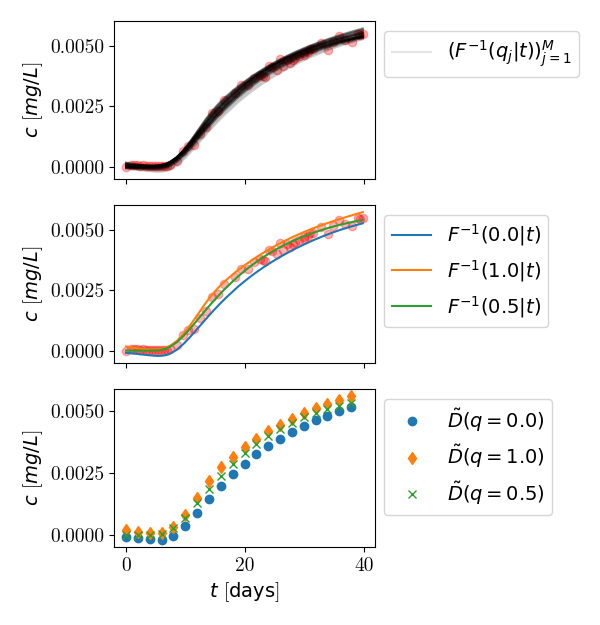
\includegraphics[width=0.9\textwidth]{figs/btc_dataspan_quantiles.png}
    \label{fig:btc_dataspan_quantiles}
    \caption{Left: BTC quantile functions for all quantile samples $q_j$. Middle: BTC quantile functions for quantiles $0$, $0.5$, and $1$. Right: BTC datasets for quantiles $0$, $0.5$, and $1$.}
\end{figure}



\section{Data and Setup}

\subsection{Experimental Setup}
The experiments were conducted using Python 3.11.3. Modified versions of the FINN code from \textcite{finn} and the PI3NN code from \textcite{pi3nn} were used. The code and specific library versions are available on GitHub. GNU parallel \cite{tange_2023_10199085} was used for parallel execution of experiments. % TODO: insert github link

\subsection{Data Acquisition}
The BTC data was obtained from the work by \textcite{finn}, originally sourced from \textcite{nowak2016entropy}. Synthetic data was generated using the same solver employed by FINN, ensuring consistency in the experimental setup.

\subsection{Training Details}
Early stopping was implemented to halt training when the loss plateaued. Training runs for FINN were discarded if the normalized mean squared error (NMSE) exceeded $10^{-5}$ (measured on BTC), ensuring a minimum level of accuracy in the learned retardation function.

\begin{equation*}
    \text{NMSE}(y, \hat{y}) = \text{MSE}(y, \hat{y}) / \text{mean}(y)
\end{equation*}




\section{Experiments}

\subsection{SPAN}
The hyperparameters that were used differ for the synthetic data case and the experimental data case:

\begin{table}[h!]
    \centering
    \begin{tabular}{>{\raggedleft\arraybackslash}m{3.5cm} | >{\raggedright\arraybackslash}m{3cm} >{\centering\arraybackslash}m{2.5cm} >{\centering\arraybackslash}m{2.5cm}}
        \toprule
        \textbf{Hyperparameter} & \textbf{Description} & \textbf{Experimental} & \textbf{Synthetic} \\
        \midrule
        Weight Initialization & \small{Seed for initial values for model weights} & \textcolor{green}{\checkmark} & \textcolor{green}{\checkmark} \\
        \midrule
        Training Data Mask (see \ref{fig:training_data_mask}) & \small{Seed for mask applied to training data} & \textcolor{red}{\ding{55}} & \textcolor{green}{\checkmark} \\
        \midrule
        Training Data Noise & \small{Seed for noise added to training data} & \textcolor{red}{\ding{55}} & \textcolor{green}{\checkmark} \\
        \midrule
        Max Epochs & \small{Maximum number of training iterations} & \textcolor{green}{\checkmark} & \textcolor{green}{\checkmark} \\
        \midrule
        MSE Loss Factor & \small{Factor for Mean Squared Error loss} & \textcolor{green}{\checkmark} & \textcolor{red}{\ding{55}} \\
        \midrule
        Physical Loss Factor & \small{Factor for physical loss} & \textcolor{green}{\checkmark} & \textcolor{red}{\ding{55}} \\
        \bottomrule
    \end{tabular}
    \caption{Hyperparameters for Experimental and Synthetic Settings}
    \label{tab:hparams}
\end{table}

In the experimental setting, $780$ samples were generated using the specified hyperparameters. For the synthetic experiments, the number of samples varied and is indicated in the respective figure captions for clarity and comparison within those specific contexts. The experimental results are shown in \ref{fig:span_samples}.
% TODO: synthetic results

\begin{figure}
    \centering
    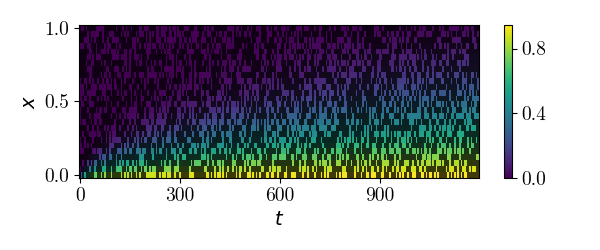
\includegraphics[width=0.9\textwidth]{figs/c_diss_field_train_random_subset.png}
    \label{fig:training_data_mask}
    \caption{Full synthetic concentration training data where 50\% of datapoints are randomly masked (dark patches).}
\end{figure}


\subsection{Data-SPAN}
This approach was applied only to the experimental data because the synthetic training data lacks noise, leading to extremely small residuals and a very narrow distribution that does not impact sampling.

For the experimental data, we sampled $70$ quantiles as detailed in \ref{sec:random_dataset_sampling}. The results are shown in \ref{fig:dataspan_samples}.



\subsection{Full-SPAN}
This approach is equivalent to Data-SPAN but additionally, for every sampled quantile, the hyperparameters are also randomly sampled. The results are shown in \ref{fig:fullspan_samples}.


\subsection{Baselines (Bayes NN via MCMC)}
We computed $10$k samples using the same parameters as \textcite{finn}; the samples are visualized in \ref{fig:mcmc_samples}.
% TODO: Why 10k? This is very important to know for arguing about efficiency.

% This is not a result (of me) thus it is here and not in the results section
\begin{figure}
    \centering
    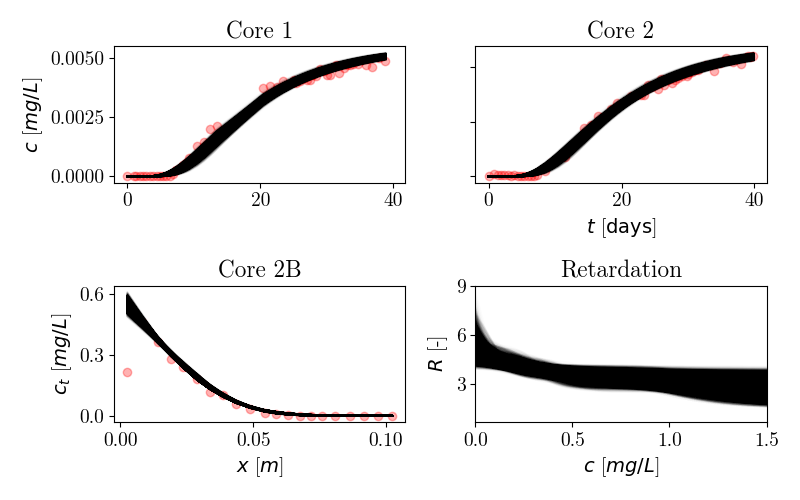
\includegraphics[width=0.9\textwidth]{figs/finn_mcmc_samples.png}
    \label{fig:mcmc_samples}
    \caption{Retardation curves generated by MCMC sampling as detailed in \ref{sec:bayes_nn}.}
\end{figure}





\section{Results}
\subsection{Samples and PIs}
\subsubsection{Synthetic Data}

\paragraph{SPAN}
When the hyperparameters are randomly sampled to learn different retardations, the uncertainty in $R(c)$ is very small as can be seen in Figure \ref{fig:synthetic_SPAN_factors_PIs}, even when all hyperparameters are combined in "All UQ".

% TODO: Get rid of upper right triangle
\begin{figure}
    \centering
    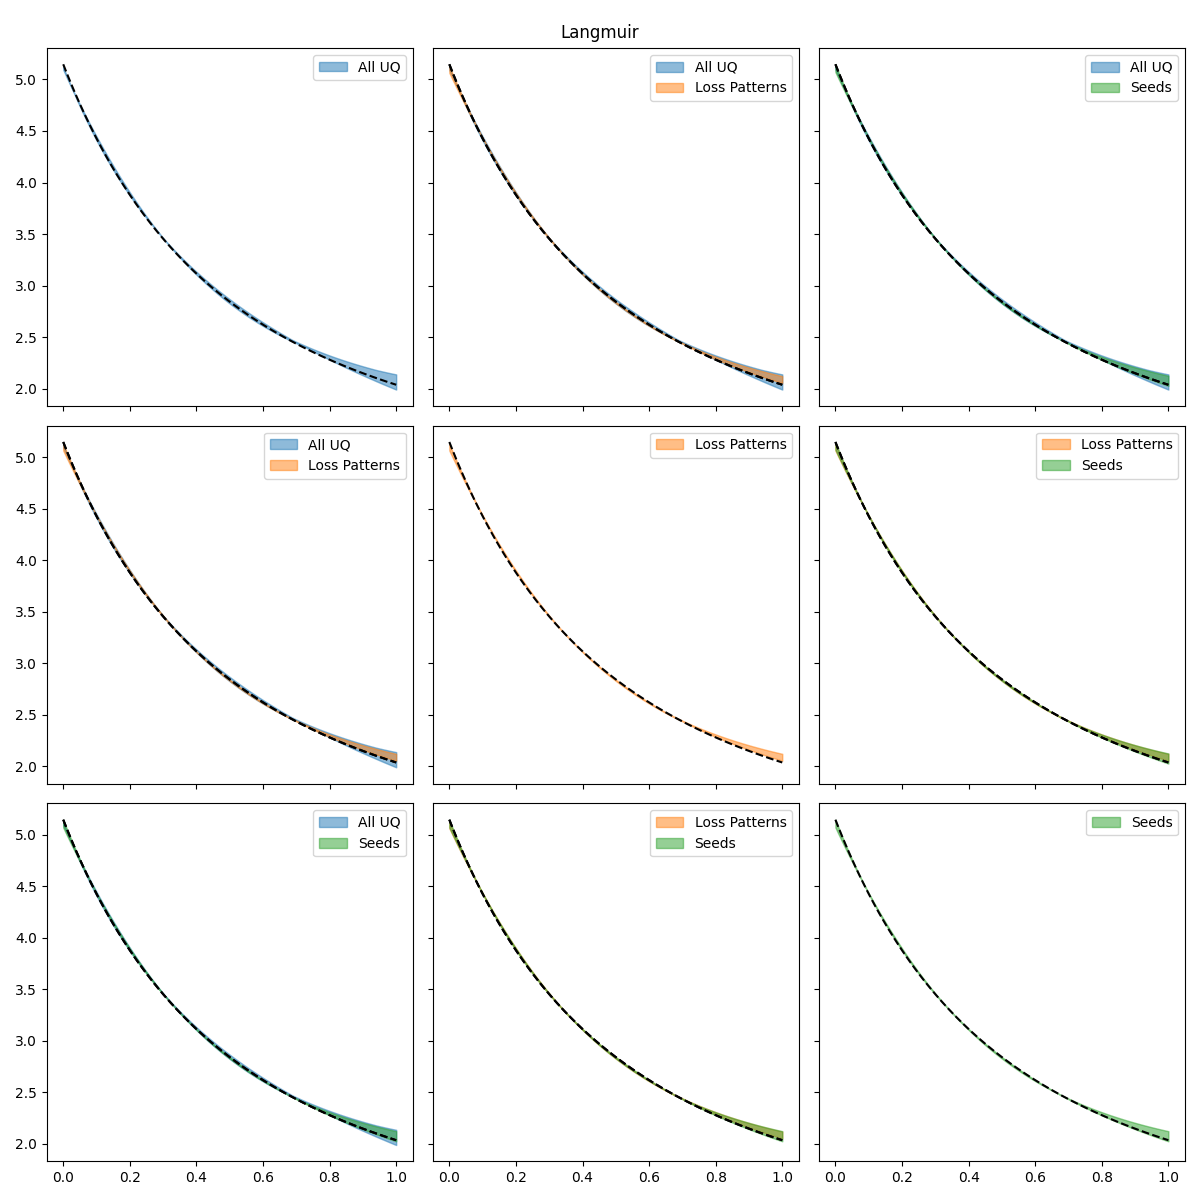
\includegraphics[width=0.9\textwidth]{figs/finn_synthetic_SPAN_factors_PIs.png}
    \label{fig:synthetic_SPAN_factors_PIs}
    \caption{Comparison of retardation PIs obtained via SPAN on synthetic data (generated by langmuir isotherm).}
\end{figure}

\paragraph{Data-SPAN}
When applying gaussian noise of the same strength as the experimental data has due to measurement error \cite{nowak2016entropy}, the uncertainty in $R(c)$ becomes much larger compared to SPAN as can be seen in Figure \ref{fig:synthetic_langmuir_c_noise}.

\begin{figure}
    \centering
    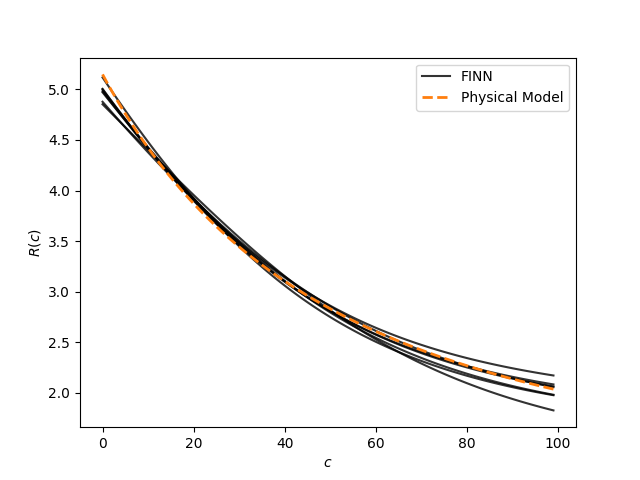
\includegraphics[width=0.9\textwidth]{figs/finn_synthetic_langmuir_c_noise.png}
    \label{fig:synthetic_langmuir_c_noise}
    \caption{Retardations learned by FINN on synthetic dataset (generated by langmuir isotherm) pertubed by gaussian noise.}
\end{figure}



\subsubsection{Experimental Data}

Figure \ref{fig:mcmc_vs_fullspan} illustrates that the 90\% prediction intervals (PIs) for both the Markov Chain Monte Carlo (MCMC) and full SPAN methods encompass similar concentration values. This agreement arises from their comparable coverage of $R(c)$ values when $c \leq 1$. While the methods diverge for larger values of $c$, this discrepancy has minimal impact on the concentration fields, as these are less sensitive to $R(c)$ in that regime. Given that full SPAN produces similar $c$ PIs but incorporates larger uncertainty in $R$, it provides a more robust uncertainty estimate. A more quantitative exploration of these findings is presented in the following sections.


\begin{figure}
    \centering
    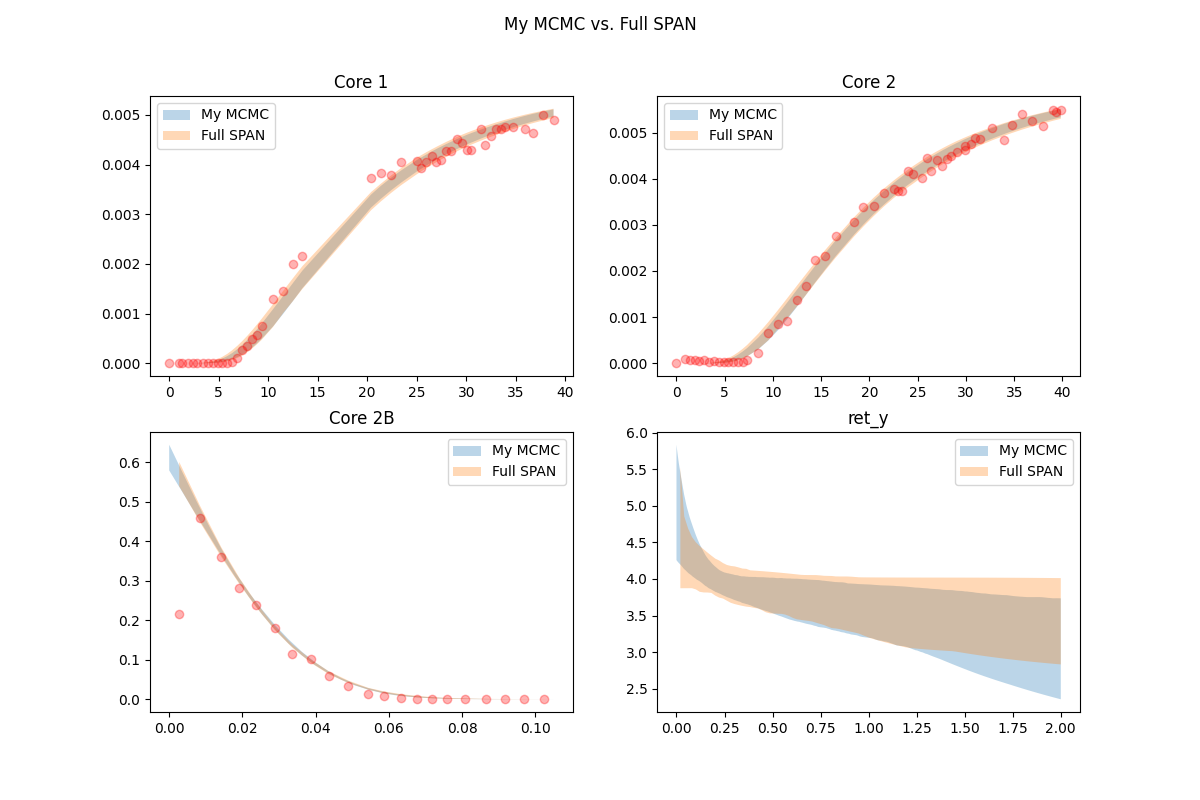
\includegraphics[width=0.9\textwidth]{figs/finn_My MCMCvsFull SPAN_PIs.png}
    \label{fig:mcmc_vs_fullspan}
    \caption{Retardation PIs and correspoding concentration PIs obtained from it by training FINN with random hyperparameters and random datasets using PI3NN (orange). Compared with MCMC approach (blue). (90\% PIs are depicted.)}
\end{figure}


\begin{figure}
    \centering
    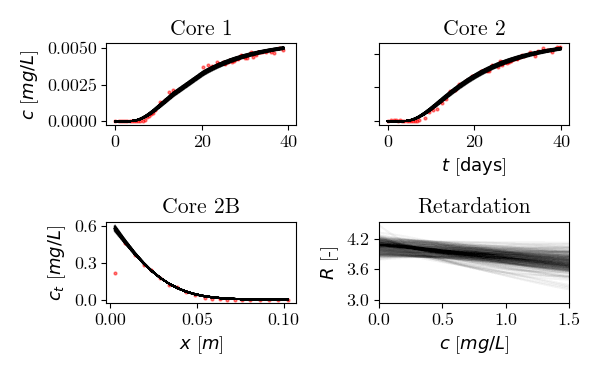
\includegraphics[width=0.9\textwidth]{figs/finn_span_samples.png}
    \label{fig:span_samples}
    \caption{Retardation samples and correspoding concentration curves obtained from it by training FINN with random hyperparameters.}
\end{figure}

\begin{figure}
    \centering
    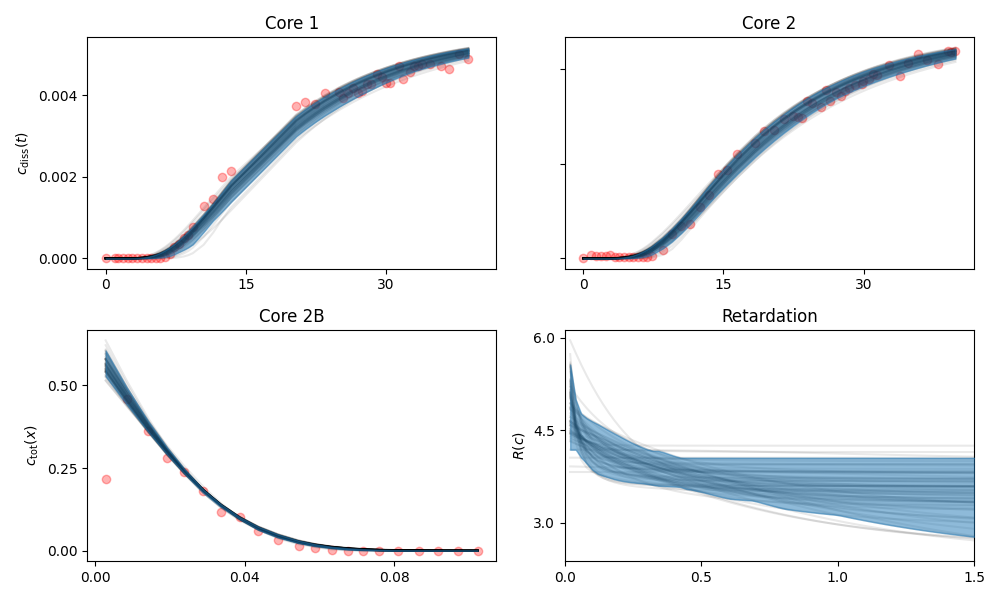
\includegraphics[width=0.9\textwidth]{figs/finn_dataspan_samples.png}
    \label{fig:dataspan_samples}
    \caption{Retardation samples and correspoding concentration curves obtained from it by training FINN with random datasets using PI3NN.}
\end{figure}

% TODO: Simulations for this have not been done yet.
\begin{figure}
    \centering
    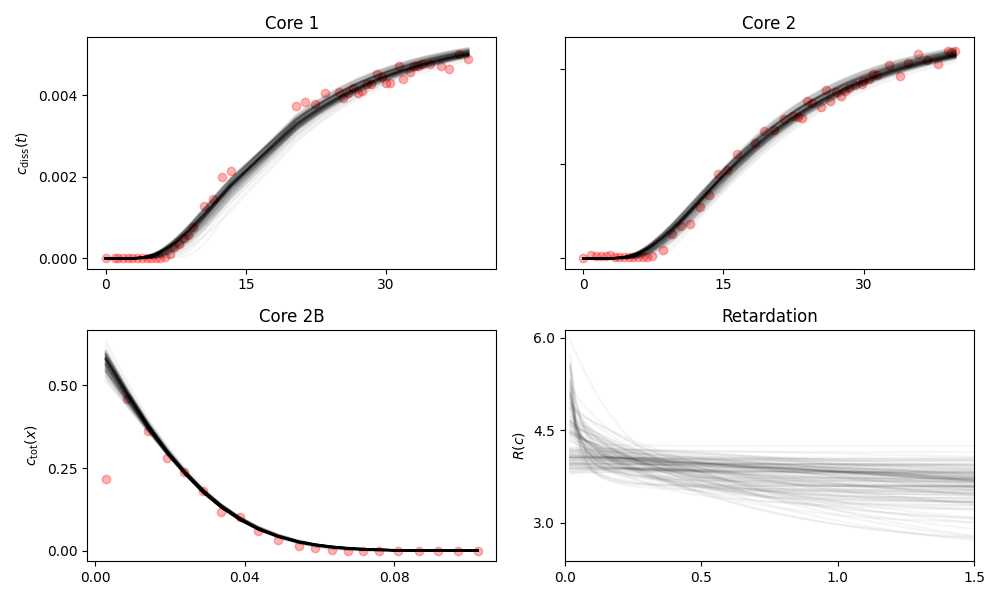
\includegraphics[width=0.9\textwidth]{figs/finn_fullspan_samples.png}
    \label{fig:fullspan_samples}
    \caption{Retardation samples and correspoding concentration curves obtained from it by training FINN with random hyperparameters and random datasets using PI3NN.}
\end{figure}




\subsection{Runtime}
We measure and compare the runtime of generating a single sample of our method and the baseline. Since SPAN as well as Data-SPAN require training of the NN from scratch for each sample, the runtime approximately equals the training time. Averaging over $10$ trials, the runtime is $170$ seconds.

The MCMC method uses thinning, saving only every $10$th sample. The average runtime for this is about $11.4$ seconds, almost $15$ times faster than our method.
% TODO: But how many samples does each method need?
% TODO: And what if the log posterior trace plot is still decreasing? Am I even allowed to take samples from it then?
% TODO: What about parallelization? Our method is trivially paralellizable. What about MCMC with Barker sampler?
% TODO: What about other problems (with e.g. more weights). Does our method get better then?



% Bit unnecessary plot?
\begin{figure}
    \centering
    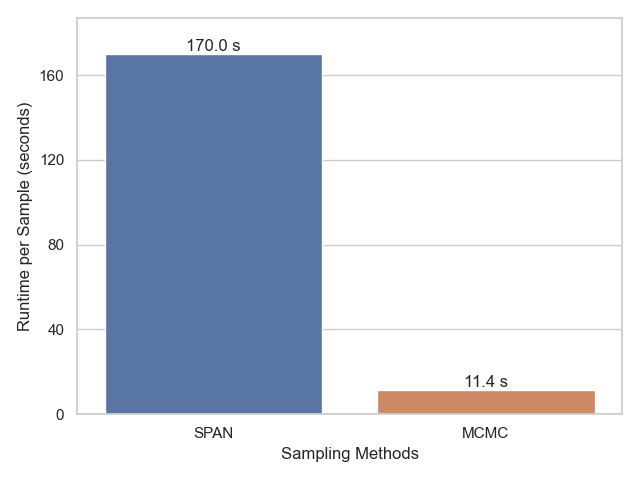
\includegraphics[width=0.9\textwidth]{figs/runtime_per_sample.png}
    \label{fig:runtime_per_sample}
    \caption{Runtime for generating a single sample using SPAN (left bar) and MCMC (right bar). Measured on the same machine and averaged over $10$ trials. Variance is too insignificant to matter here.}
\end{figure}

\subsection{Likelihood}
To evaluate the predictive quality of our method, we use its samples to estimate a probability distribution. This is done by computing a histogram. We can then estimate the likelihood of the training data $\mathcal{D}$ given this distribution. We transform the likelihood into a negative log-likelihood (NLL) to obtain more accurate results. A lower NLL is better. Applying this procedure on SPAN yields a NLL of $-6.41$, $-7.11$ for MCMC, and $-7.14$ for Data-SPAN. A good baseline to compare this against, is a normal distribution around the FINN BTC prediction mean and standard deviation equal to the sample standard deviation computed from the residuals:
\begin{equation*}
    p(c; t) = \frac{1}{\sqrt{2 \pi \mathcal{s}^2}} \exp(-\frac{1}{2 \mathcal{s}^2} (\hat{c}(x=L, t; \theta_{\mathcal{D}}) - c)^2)
\end{equation*}
This yields a NLL of $-7.50$, which is the lowest value. % TODO: Interpretation

\subsection{Reliability Curve}
Another quantification done by \textcite{finn} is the average calibration of the PI. This can be visualized using the reliability curve.

The reliability curve assesses the calibration of predicted confidence intervals. It plots the observed frequency of the true value falling within a given confidence interval against the predicted confidence level. To compute it, the prediction range is divided into bins (e.g., by confidence levels). For each bin, the proportion of predictions where the true value falls within the corresponding PI is calculated. Ideally, the curve should follow the diagonal line (perfect calibration). A curve above the diagonal indicates underconfidence (the true value falls within the PI more often than predicted), while a curve below the diagonal indicates overconfidence.

The results, shown in Figure \ref{fig:reliability_curves}, suggest that Data-SPAN provides the best calibrated PI. Overall, all methods are generally overconfident, SPAN the strongest. Only Data-SPAN is a little underconfident for very small $c$ values.

\begin{figure}
    \centering
    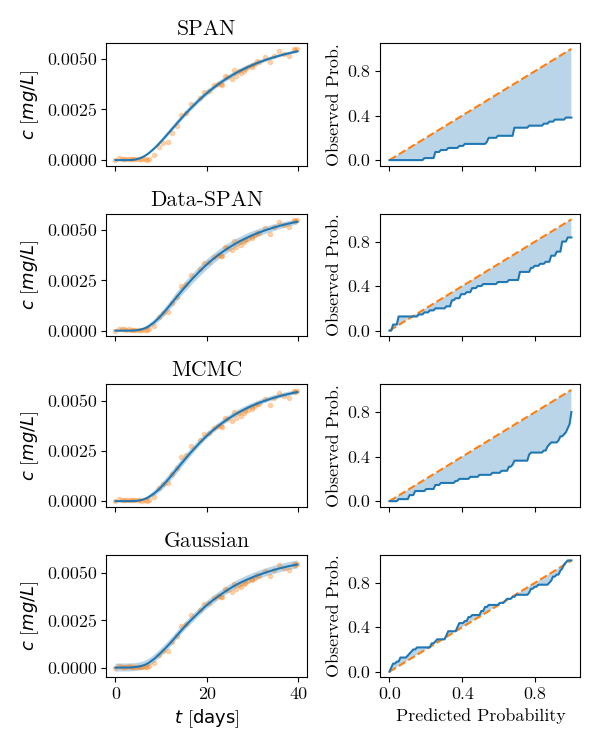
\includegraphics[width=0.9\textwidth]{figs/reliability_curves.png}
    \label{fig:reliability_curves}
    \caption{Top: Core 2 BTC 90\% PIs for the different methods (SPAN, Data-SPAN, MCMC). Bottom: Reliability curve for each method.}
\end{figure}


\subsection{Sensitivity Analysis}
\label{sec:sensitivity}
Sensitivity analysis investigates how variations in input parameters affect the model output. Unweighted SPAN samples inherently perform sensitivity analysis because each sample represents a different set of hyperparameters, and the resulting retardation function and its impact on the concentration field demonstrate the influence of those hyperparameters.

One sensitivity analysis method is based on standardized regression coefficients, sometimes referred to as beta coefficients or beta weights. They represent the relative importance of each predictor variable (hyperparameter $h$ in this case) in explaining the variance of the outcome variable ($R(c)$).
Importantly, the sum of these normalized coefficients can exceed 1 as parameters may explain common variances. The value shows how important the respective parameter is in relation to the rest.
Since these parameters are based on linear regression, they should be interpreted with caution, especially when non-linear relationships exist between the hyperparameters and the retardation function.

We average the importance for $R(c)$ over a set of $c$ values and obtain $0.033$ for \textbf{Physical Loss Factor}, $0.051$ for \textbf{Weight Initialization}, $0.159$ for \textbf{MSE Loss Factor}, and $0.570$ for \textbf{Max Epochs}.

This indicates that \textbf{Max Epochs} and \textbf{MSE Loss Factor} have the largest impact on $R(c)$ overall. The seed used for weight initialization and the physical loss factor play only negligible roles.

Figure \ref{fig:sensitivity} shows the relative importance for values of $c$ over which the average was taken.


\begin{figure}
    \centering
    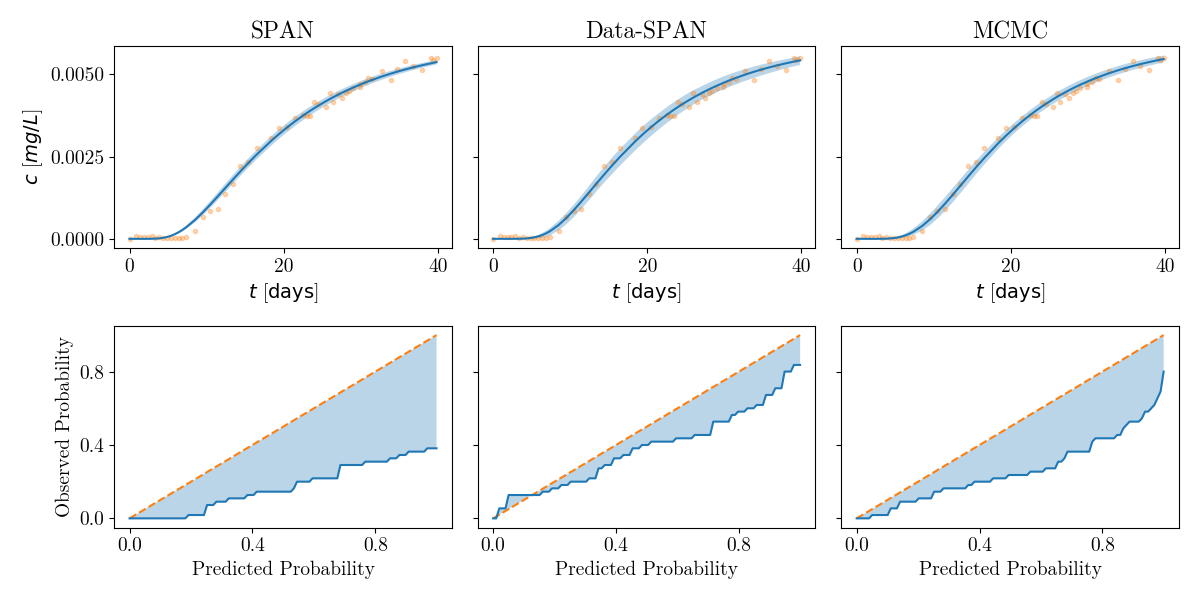
\includegraphics[width=0.9\textwidth]{figs/sensitivity.png}
    \label{fig:sensitivity}
    \caption{Relative importance on the variance of $R(c)$ of each hyperparameter for different values of $c$.}
\end{figure}



\section{Discussion}
\subsection{Retardation Range} % TODO: better name?
For some $c$ $R(c)$ does not affect the whole $c$ field equally. This can be seen by looking at figure \ref{fig:triangle_ret_pertubation} which shows constant retardation curves that are pertubed additively by triangle functions with centers at different $c$ values. With increasing $c$ center, the error caused by the hat functions goes quickly to zero. For $c > 1$, the error becomes zero. This is because the concentration field $c(x,t)$ only contains values between $0$ and $1$. But there is also a noticeable difference between the maximum error measured on the full field vs. the BTC. The BTC error is consistently much lower.
The full field error can not be detected in the case of experimental data as there is no access to the full field solution. For this reason, the range of $c$ values for which significant statements about the uncertainty of $R(c)$ can be made, is restricted to a narrow range. The exact range is difficult to estimate as the stength of influence for different retardations is unclear.


\begin{figure}
    \centering
    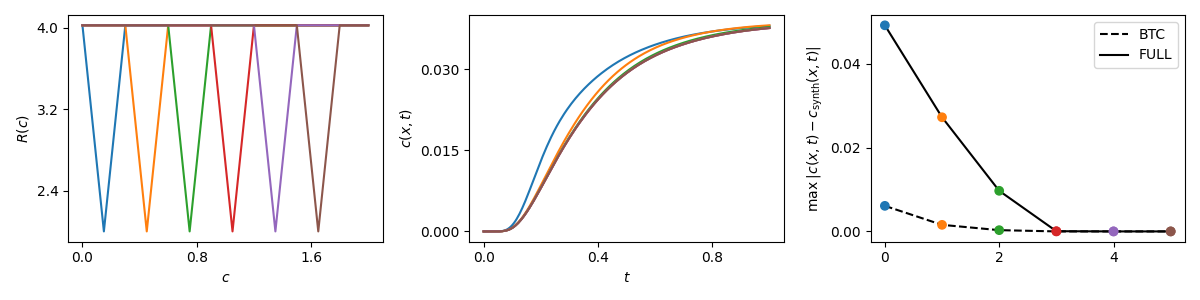
\includegraphics[width=0.9\textwidth]{figs/triangle_ret_pertubation.png}
    \label{fig:triangle_ret_pertubation}
    \caption{Left: Retardations with triangle peaks. Middle: Concentration BTC for these Retardations. Right: MAE for each on the full field and BTC.}
\end{figure}


\subsection{Samples and PIs}
The analysis of our results reveals several key insights regarding the performance and characteristics of the different uncertainty estimation methods, particularly focusing on the comparison between Full-SPAN and Markov Chain Monte Carlo (MCMC).

Firstly, the synthetic data case exhibits significantly lower uncertainty compared to the experimental data scenario. This can be attributed to several factors: a larger number of datapoints, which reduces epistemic uncertainty; the reduced effectiveness of Data-SPAN due to the absence of noise in the synthetic data; and the utilization of less effective SPAN hyperparameters (such as excluding the strongest options like "Max Epoch" or "MSE loss factor," as shown in Section \ref{sec:sensitivity}).

Interestingly, Data-SPAN does not demonstrate a substantial improvement in uncertainty estimation with an increasing number of samples, especially when compared to MCMC. This is a favorable characteristic, as it implies that Data-SPAN can achieve reliable uncertainty estimates even with a limited number of samples and thus computational effort. Furthermore, SPAN benefits from trivial parallelizability, unlike MCMC, which requires sequential sampling or more advanced methods. This, coupled with Data-SPAN's ability to operate effectively with fewer samples, establishes SPAN as a more computationally efficient method for uncertainty quantification.
% TODO: I don't like how I sometimes use SPAN but mean Full-SPAN and stuff like this. Maybe I should introduce Para-SPAN and get rid of Full-SPAN?
% TODO: Btw, I remember that I was told not to use the word "parameter" because this can be confused with something else.

Although our sensitivity analysis indicated that certain hyperparameters exerted minimal influence on the results, their inclusion does not negatively impact performance. This is because Monte Carlo sampling, the core technique employed here, is inherently independent of dimensionality.

Finally, a comparison of the prediction intervals (PIs) generated by Full-SPAN and MCMC, specifically the $R(c)$ PI, and their respective likelihoods, reveals comparable performance. Qualitatively, both methods appear to achieve a similar level of accuracy in capturing uncertainty.




\subsection{Limitations}
One limitation of our approach lies in its "brute-force" nature, not only due to the computational effort but also due to the process itself. While we gain insights into uncertainty, the obtained result is highly dependent on the used solver and selected hyperparameters in the case of SPAN and highly depdendent on the given dataset in the case of Data-SPAN. Ideally, uncertainty is a byproduct of the method and the uncertainty in the data.

Furthermore, the weighting process raises concerns. The BTC is constrained to a small subset of concentration values compared to the full field (only 0 to 0.04 instead of 0 to 1.0). This raises questions about the validity of weighting e.g. $R(c=0.0)$ samples the same way as $R(c=1.0)$, as the latter do not directly influence the predicted BTC and thus their likelihood contribution is questionable.


\section{Conclusion}
\subsection{Summary}
This work investigated uncertainty quantification (UQ) for the retardation factor in a diffusion-sorption process using the FINN framework. We proposed two novel UQ methods, SPAN and Data-SPAN, based on perturbing hyperparameters and training data, respectively. Empirical analysis demonstrated the near-uniqueness of the inverse problem, enabling the interpretation of the UQ results. While computationally more expensive than MCMC, our methods offer a different perspective on uncertainty by directly exploring the effects of various uncertainties within the training data and solver process.

\subsection{Future Work}
% TODO


\section{References}
\printbibliography


\end{document}
